% !TEX root =  main.tex

\section{Empirical Verification and Applications}
\label{sec:empirical}

The convergence rates proven in Section~\ref{sec:convergence} are only
\emph{upper bounds} on the worst-case performance we can expect. We will now
examine whether these convergence rates are tight in practice, investigate what happens
when our guidelines are not followed, and outline some possible applications of NMC. 

\subsection{Simple Analytic Model}
\label{sec:simple}

We start with the following simple analytically calculable problem
\begin{equation}
\begin{aligned}
\label{eq:model}
& y \sim \mathrm{Uniform}(-1,1), &&
z \sim \mathcal{N}(0,1), \\
& \phi(y,z) = \sqrt{2/\pi}\exp\left(-2(y-z)^2\right), &&
f(y,\gamma(y)) = \log (\gamma (y)) = \log(\E_z[\phi(y,z)]).
\end{aligned}
\end{equation}
for which $I = \mathbb{E}_{y \sim p(y)}\left[f\left(y,\mathbb{E}_{z\sim p(z|y)}\left[\phi(y,z)\right]\right)\right]=\frac{1}{2}\left(\log(2)-\log(5)-\log(\pi)\right)-\frac{2}{15}$.
Figure~\ref{fig:emprical-conv} shows the corresponding empirical convergence obtained by
applying~\eqref{eq:nested-mc} to~\eqref{eq:model} directly. It shows that for this
problem the theoretical convergence rates from Theorem~\ref{the:Repeat} are indeed
realized.\footnote{Note this the continuous differentiability assumption is satisfied as $\gamma(y)\neq0$
or $\infty$ for any $y\in[-1,1]$.}
The figure also demonstrates the danger of not increasing
$M$ with $N$, showing that the NMC estimator converges to an incorrect solution when $M$
is held constant.  Figure~\ref{fig:tau_sweep} shows the effect of varying $N$ and $M$ for various
fixed sample budgets $T$ and demonstrates that the asymptotically optimal strategy can be suboptimal
for finite budgets.

\begin{figure}[t]
	\centering
	\begin{subfigure}[b]{0.49\textwidth}
		\centering
	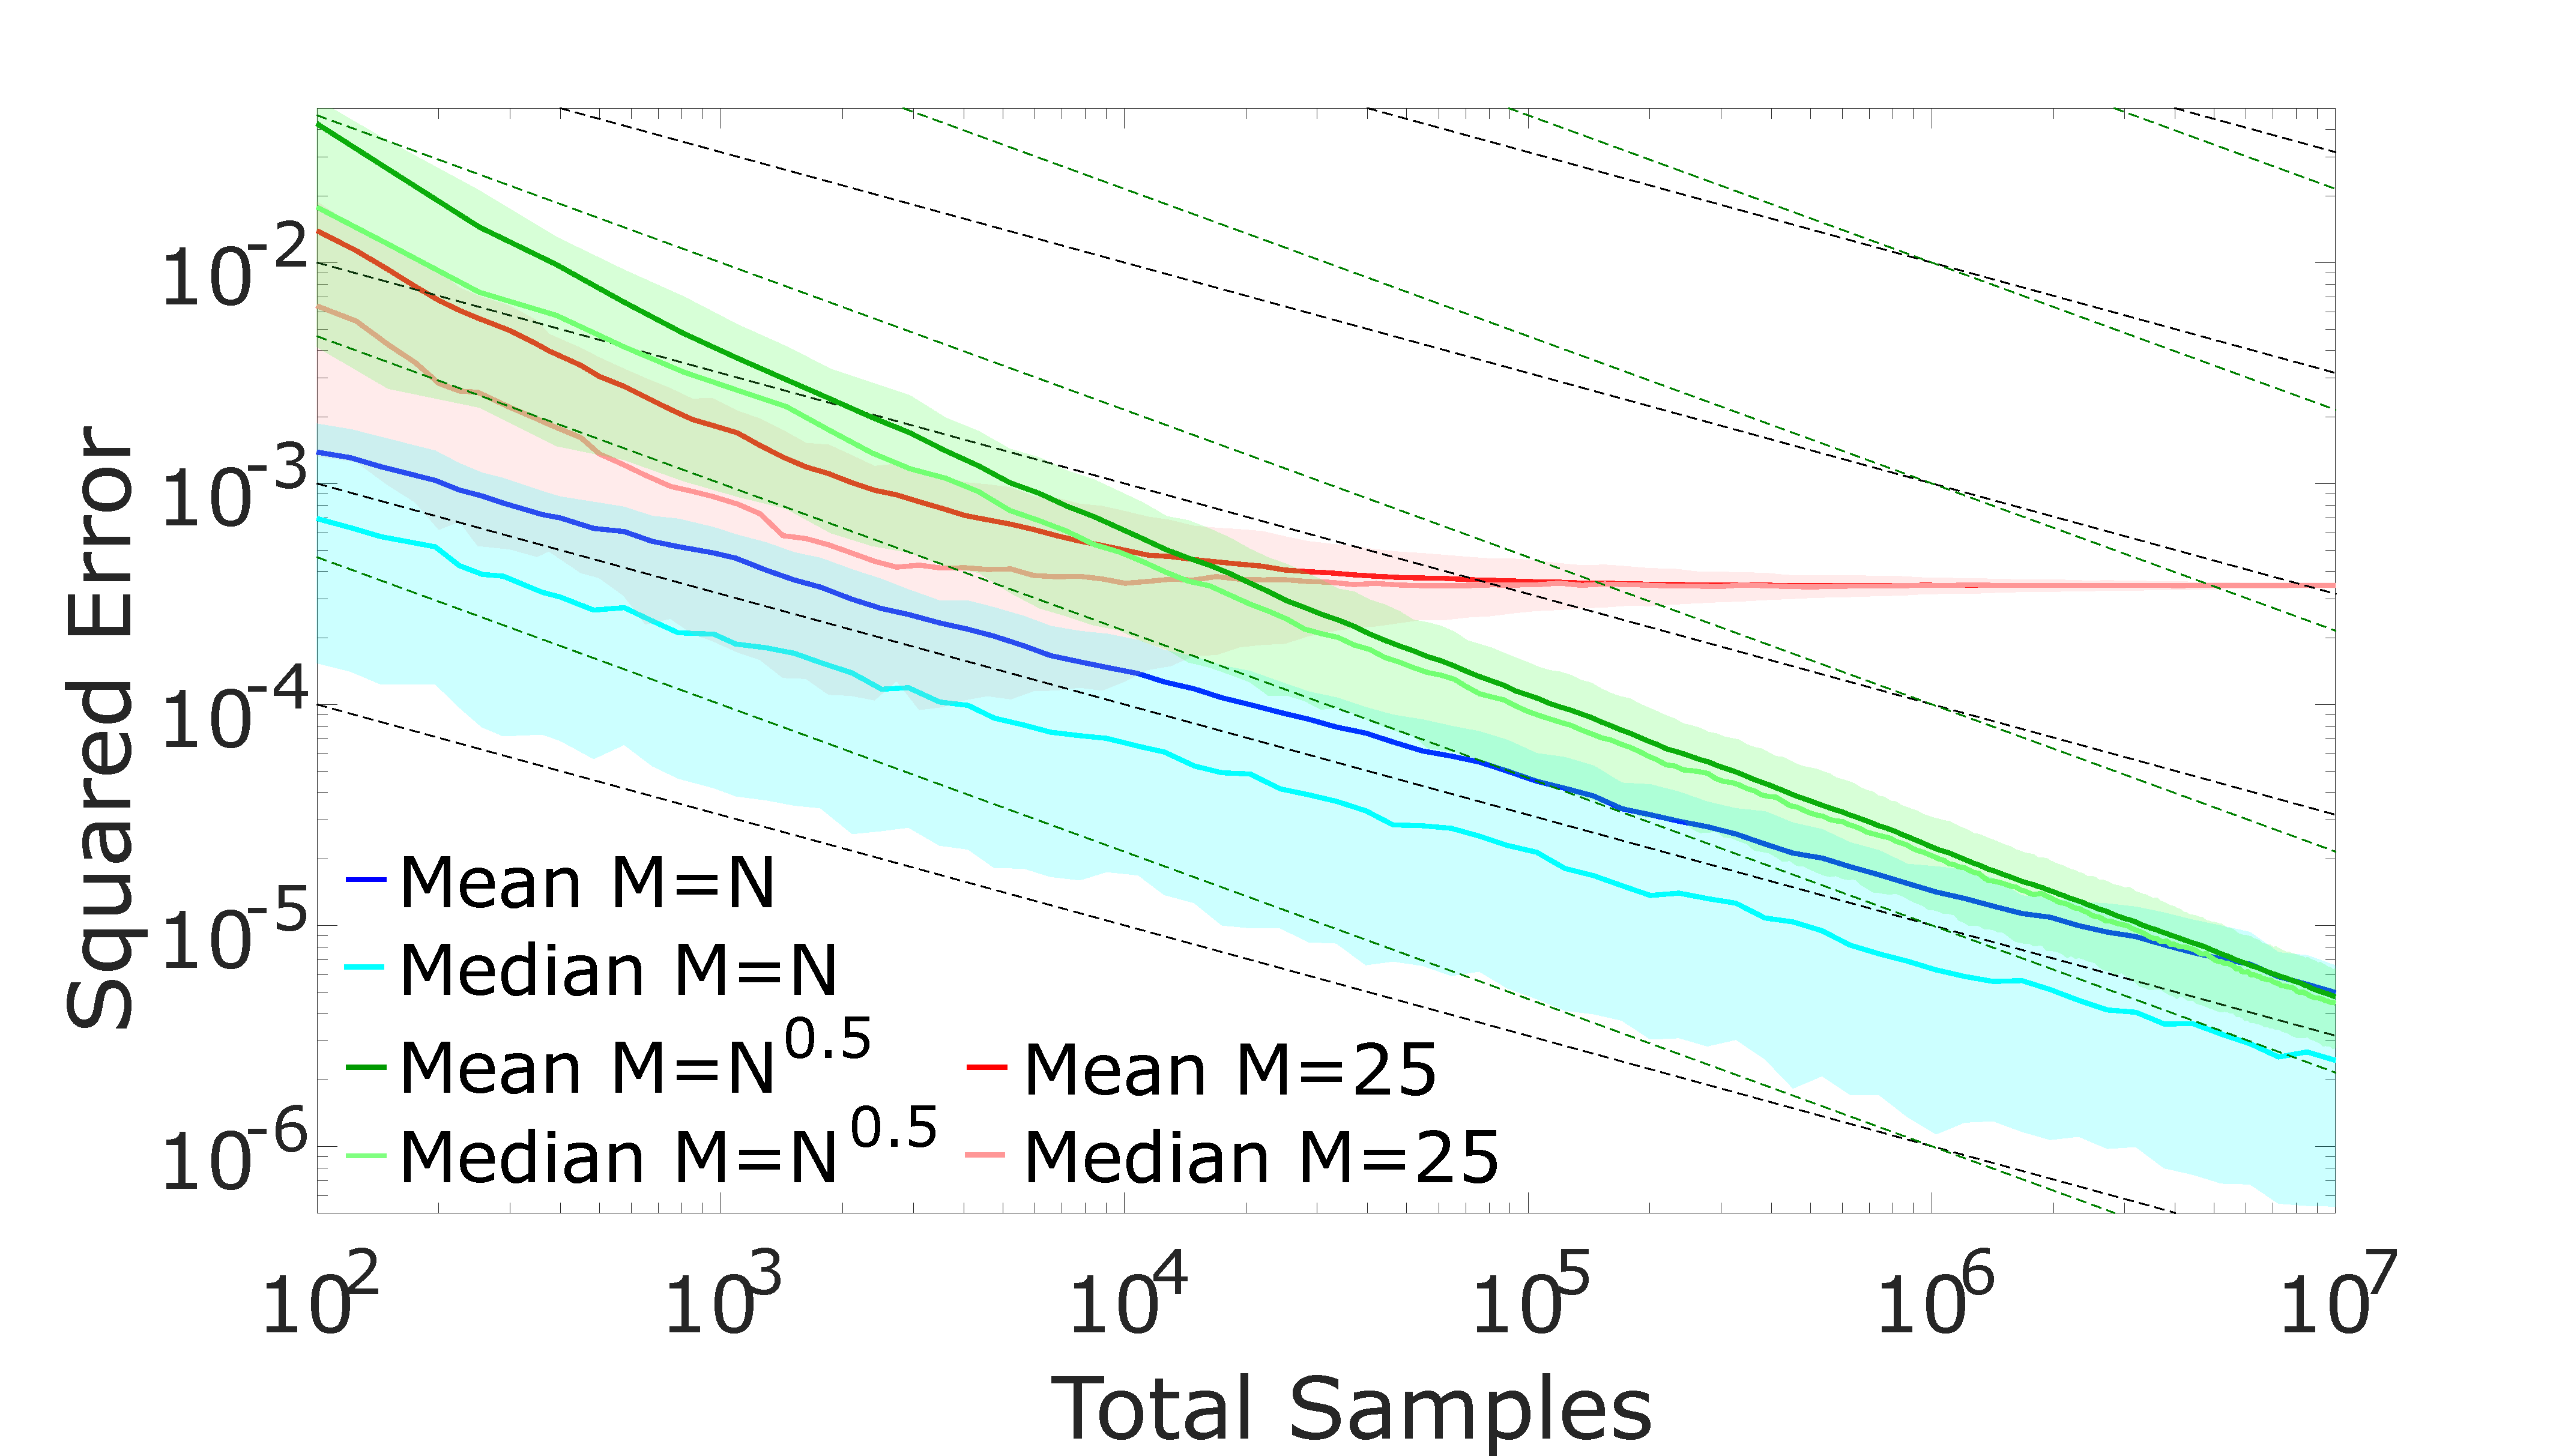
\includegraphics[width=0.99\textwidth,trim={1.5cm 0 3.5cm 0},clip]{gaussian_conv2}
	\caption{Convergence of NMC for different $\tau$. \label{fig:emprical-conv}}
	\end{subfigure}
	\begin{subfigure}[b]{0.49\textwidth}
		\centering
	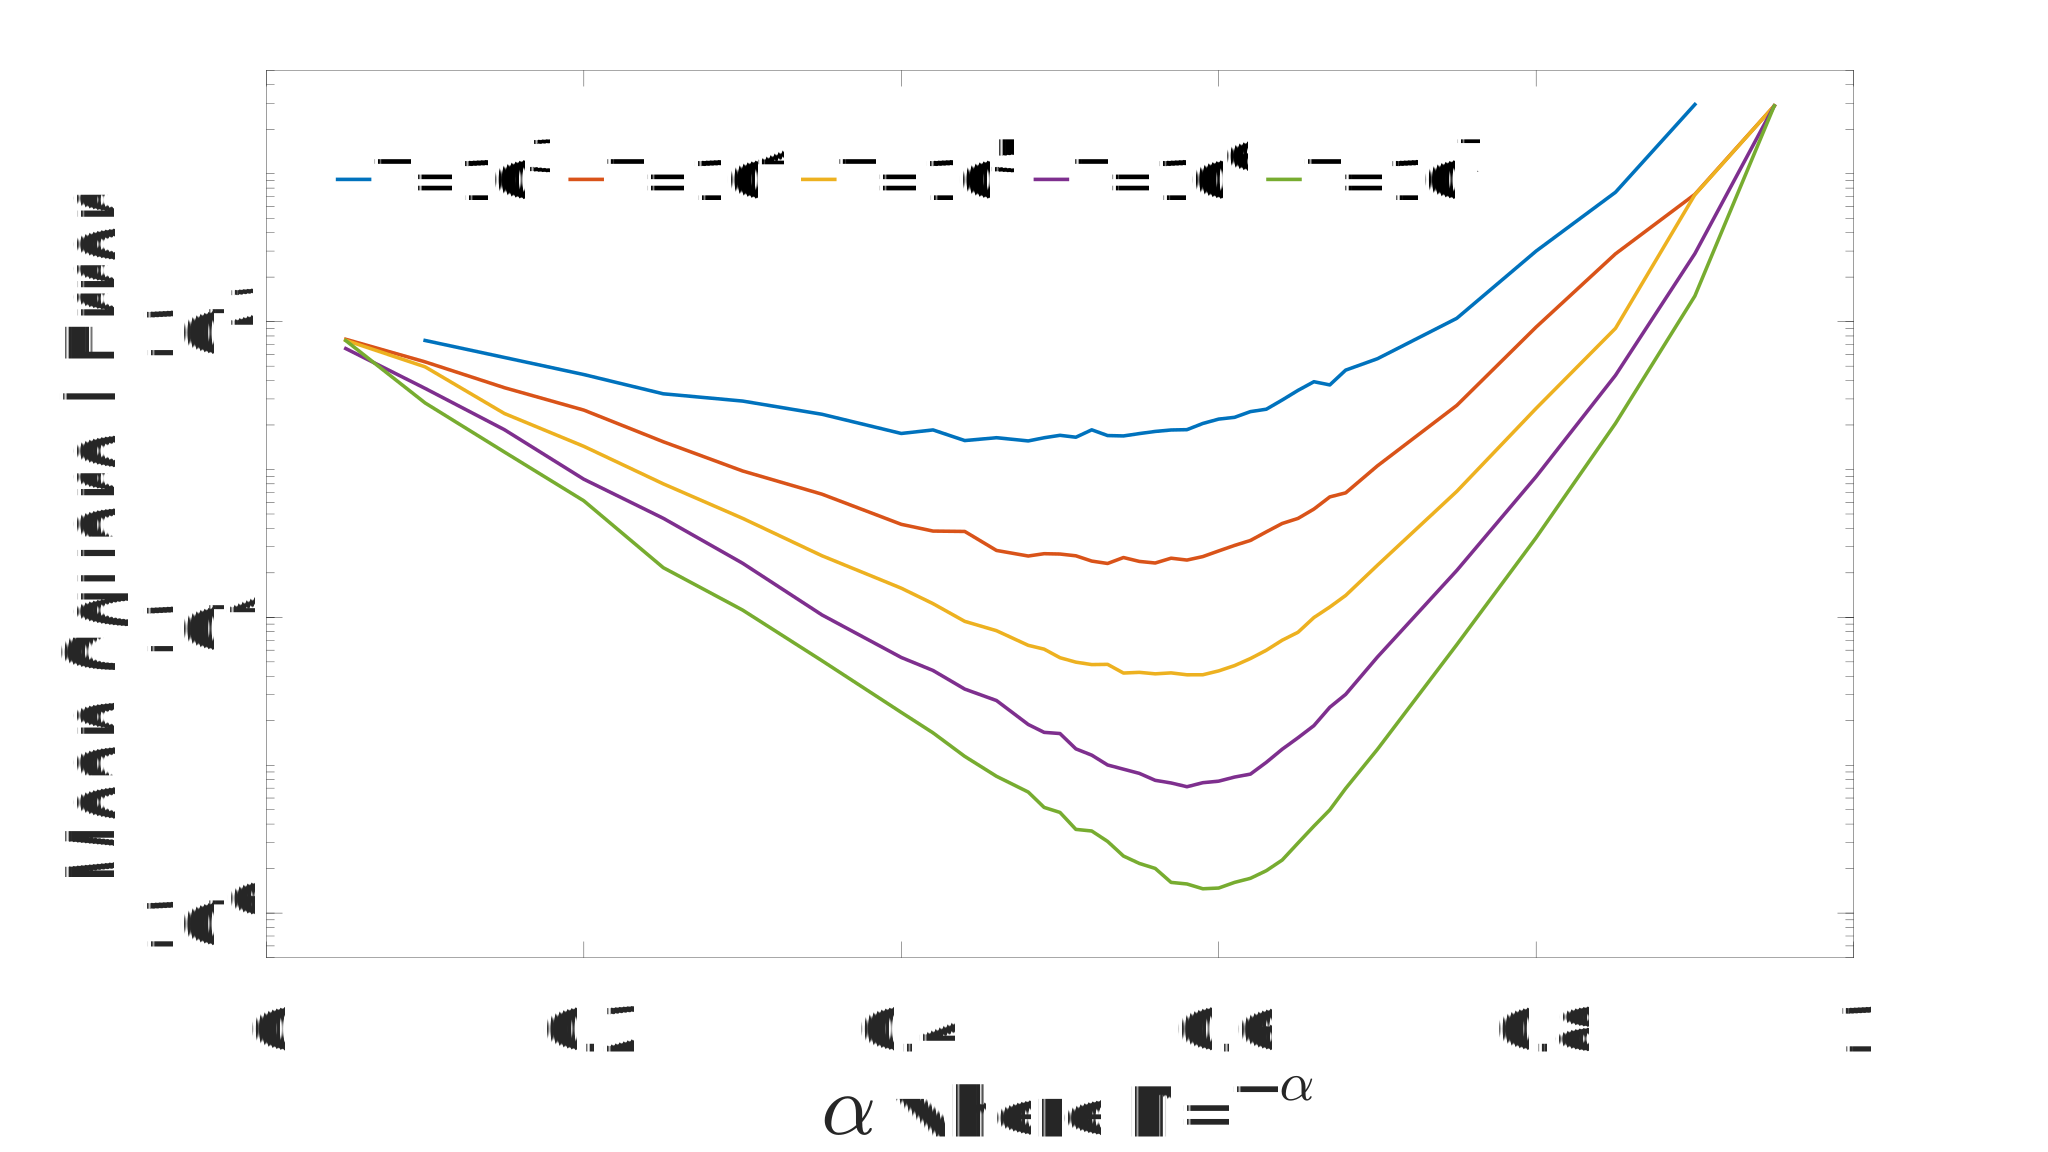
\includegraphics[width=0.99\textwidth,trim={1.5cm 0 3.5cm 0},clip]{tau_sweep}
		\caption{Final error for different $T$ and $N$.\label{fig:tau_sweep}}
	\end{subfigure}
	\caption{Empirical convergence of NMC for~\eqref{eq:model}.  Shown left is the
		convergence in total samples for different ways of setting $M$ and $N$.  
		Results are averaged over 1000 independent runs, while shaded regions give the 25\%-75\% quantiles. We
		see that the theoretical convergence rates (as shown by the dash lines) are observed. 
		The fixed $M$ case converges at the MC error rate, but to a biased solution.
		Shown right is the final error for different total sample budgets
		as a function of $\alpha$ where $N=T^{\alpha}$ and $M=T^{1-\alpha}$ iterations are used for the outer
		and inner estimators respectively.  This shows that even though $\alpha=2/3$ is the
		asymptotically optimal allocation strategy, this is not the optimal solution for
		finite $T$. Nonetheless, as $T$ increases, the optimum value of $\alpha$ increases,
		starting at around $0.5$ for $T=10^3$ and reaching around $0.6$ for $T=10^7$. \vspace{-5pt}}
\end{figure}	

% !TEX root =  main.tex

\subsection{Repeated Nesting}
\label{sec:exp-repeat-app}

We next consider some simple models with multiple levels of nesting, starting with
\begin{subequations}
	\label{eq:repeat-nest}
\begin{align}
y^{(0)} \sim \mathrm{Uniform}(0,1), \quad &
y^{(1)} \sim \mathcal{N}(0,1), \quad
y^{(2)} \sim \mathcal{N}(0,1), \displaybreak[0] \\ 
f_0 \left(y^{(0)}, \gamma_1\left(y^{(0)}\right)\right)&= \log \gamma_1\left(y^{(0)}\right) \displaybreak[0] \\ 
f_1 \left(y^{(0:1)}, \gamma_2\left(y^{(0:1)}\right)\right)&= 
\exp\left(-\frac{1}{2}\left(y^{(0)}-y^{(1)}-\log \gamma_2\left(y^{(0:1)}\right)\right)\right) \displaybreak[0] \\ 
f_2 \left(y^{(0:2)}\right)&=\exp\left(y^{(2)}-\frac{y^{(0)}+y^{(1)}}{2}\right)
\end{align}
\end{subequations}
which has analytic solution $I=\E \left[f_0 \left(y^{(0)},\E \left[f_1 \left(y^{(0:1)},\E \left[f_2\left(y^{(0:2)}\right) \middle| 
y^{(0:1)}\right]\right) \middle| y^{(0)}\right]\right)\right]=-3/32$. 
The converge plot shown in Figure~\ref{fig:multi-nest} shows that the
theoretically expected convergence\footnote{Strictly speaking the assumptions of Theorem~\ref{fig:multi-nest} are
	not actually satisfied for this model and the later modifications
	 because $K_1 = C_1 = \infty$.  However, we see convergence behavior
	as if the assumptions were satisfied.  This highlights the importance of Theorem~\ref{the:Consistent}
	because $f_1$ does satisfy this weaker assumption.}
behaviors are observed for different methods of setting 
$N_0, N_1$, and $N_2$.

\begin{figure}[t]
	\centering
	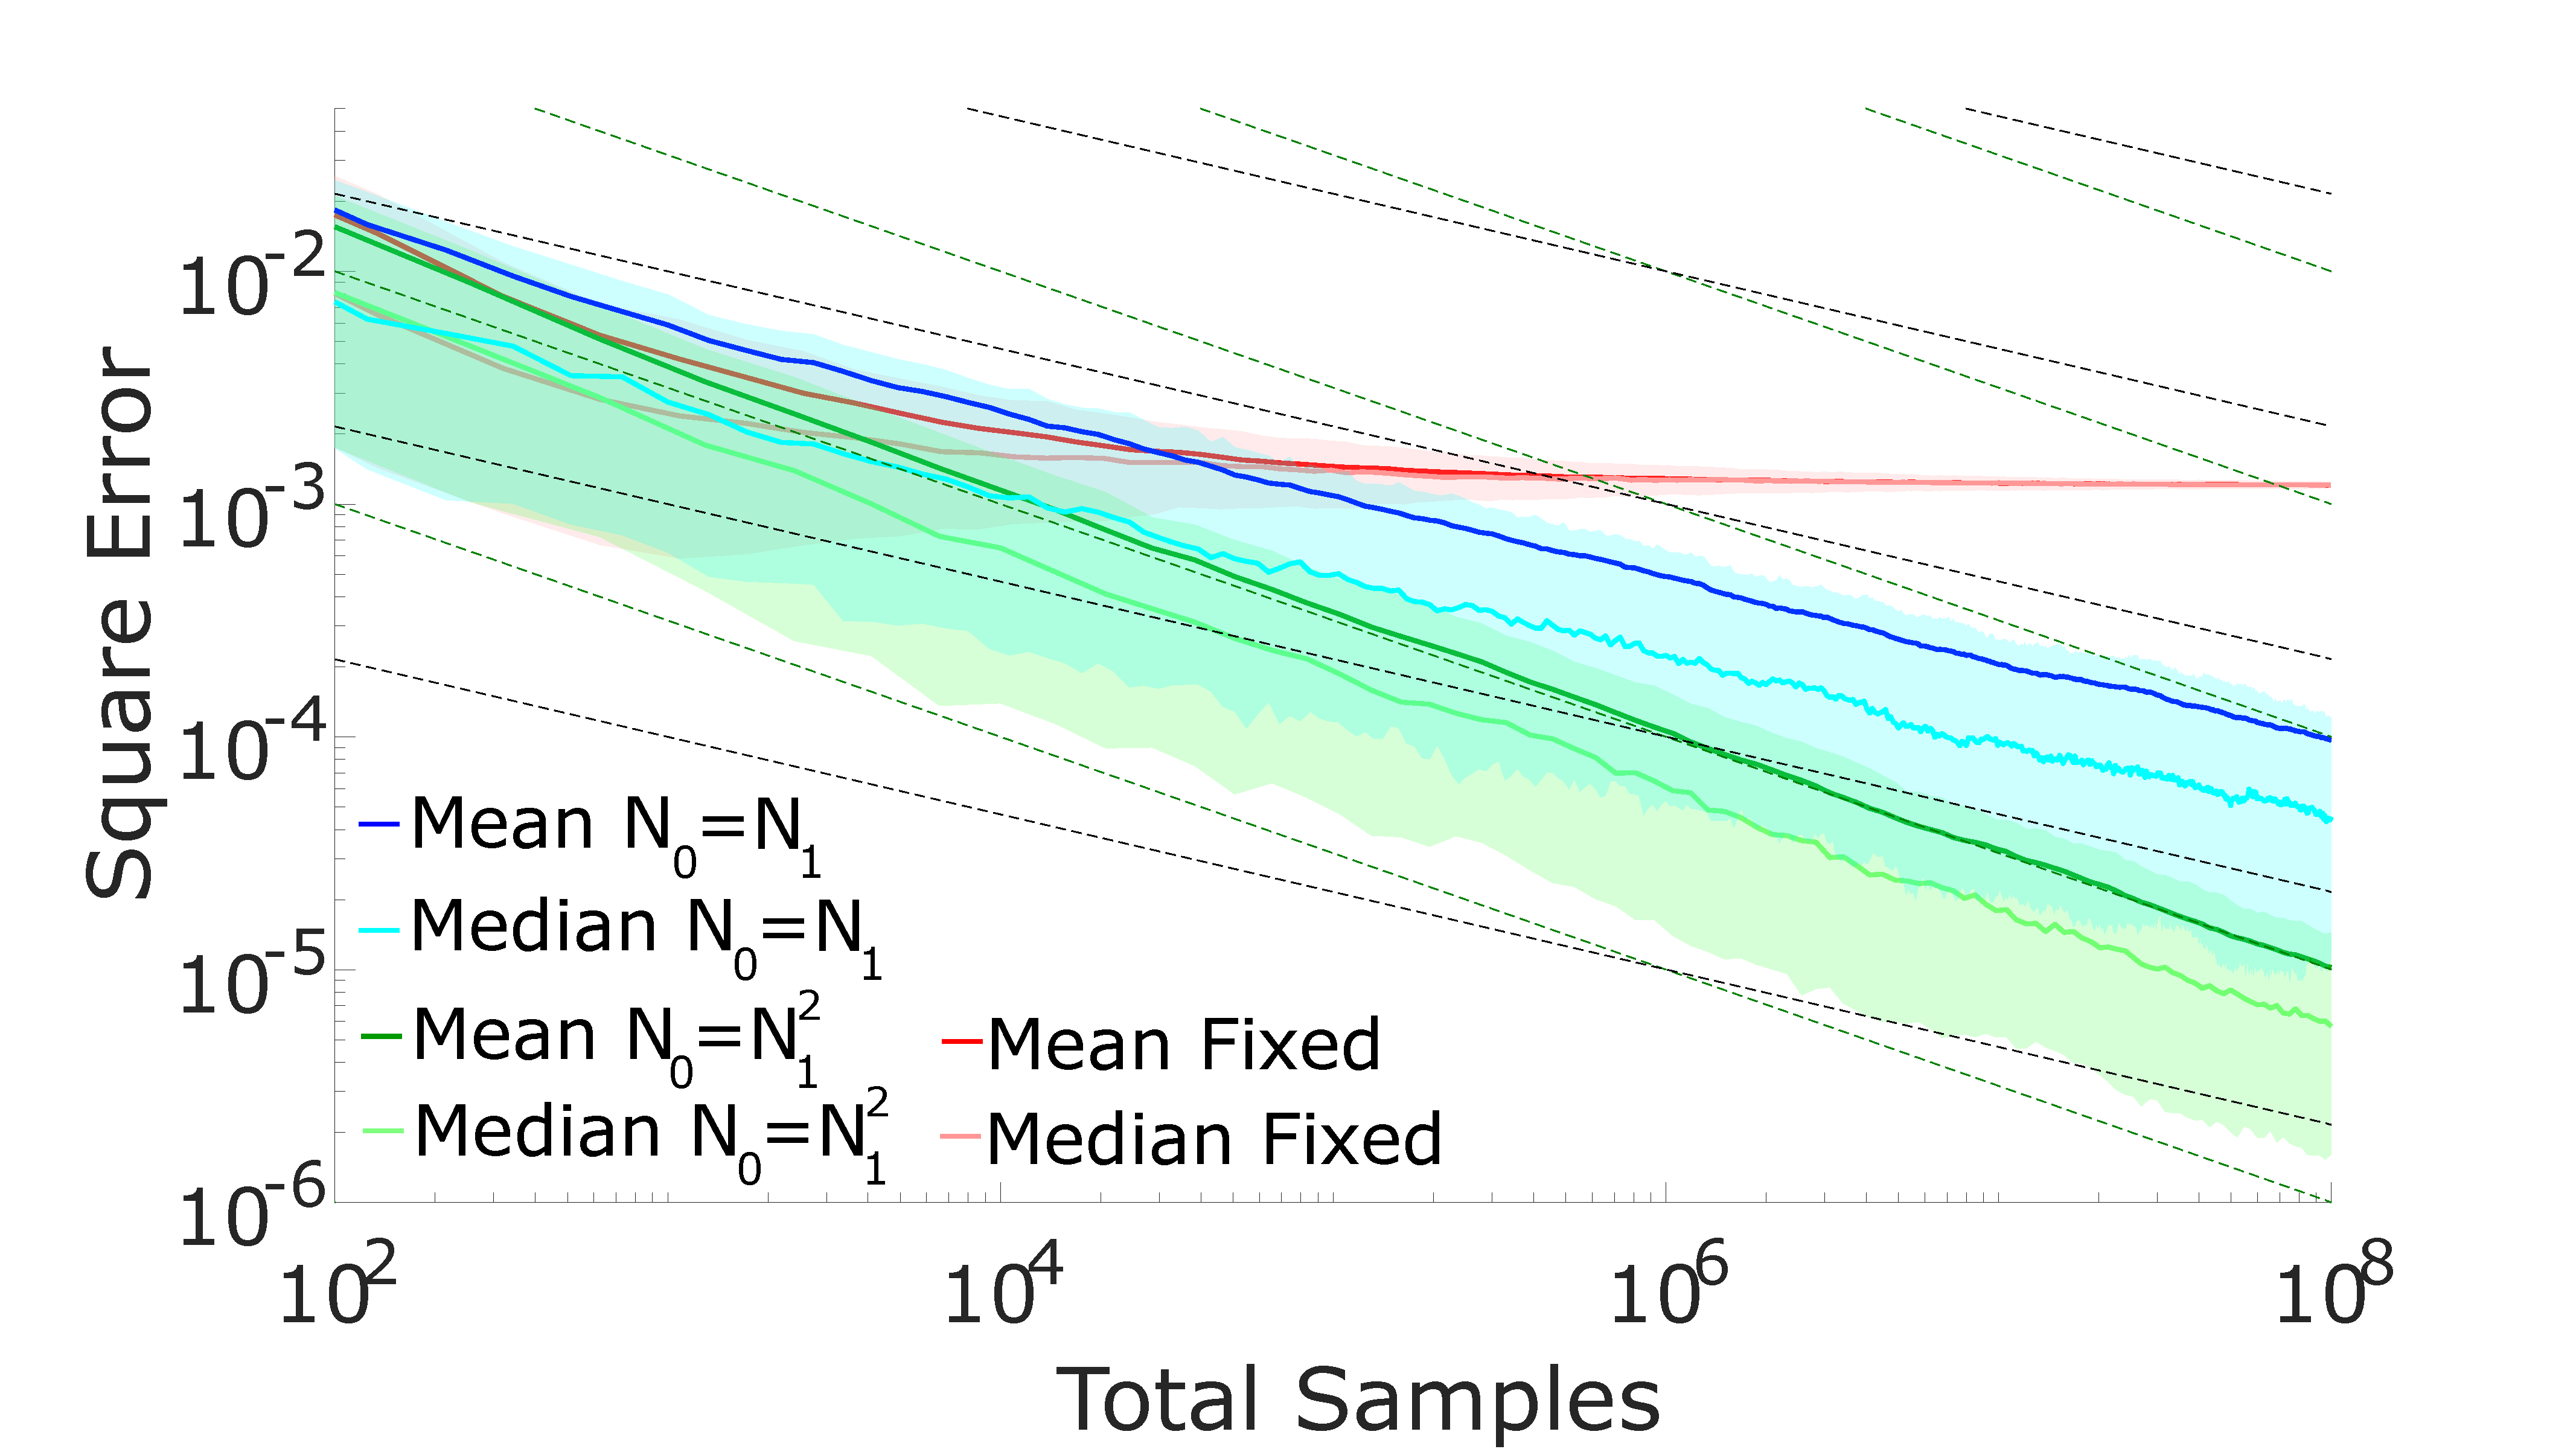
\includegraphics[width=0.5\textwidth,trim={1.5cm 0 3.5cm 0},clip]{repeat_nest_an}
	\caption{Empirical convergence of NMC to~\eqref{eq:repeat-nest} for an increasing total sample budget
		$T=N_0 N_1 N_2$.  Results are averaged over 1000 independent runs, while shaded regions give the 25\%-75\% quantiles.
		Shown in red is the convergence with a fixed $N_2=5$ and $N_1=N_2^2$, for which we see gives convergence
		to a biased solution, such that the error remains bounded as $T$ increases.  Shown in blue is the convergence
		when setting $N_0=N_1=N_2$, which we see converges at the expected $O(T^{-1/3})$ rate.  The black dashed lines
		provide a reference for this expected convergence of this estimator.  Shown in green is the convergence when
		setting $N_0=N_1^2=N_2^2$ which we seen again gives the theoretical convergence rate, this time $O(T^{-1/2})$
		with the dashed green lines providing reference.\label{fig:multi-nest}}
\end{figure}	

We next consider the empirical performance of different strategies for choosing $N_0, N_1$, $N_2$ under a 
finite fixed budget $T=N_0N_1N_2$.
To do this, we define $\alpha_1$ and $\alpha_2$ such that $N_0 = T^{\alpha_1}$, 
$N_1 = T^{\alpha_2(1-\alpha_1)}$, and $N_2 = T^{(1-\alpha_1)(1-\alpha_2)}$ and then consider the variation in the
mean squared error with $(\alpha_1,\alpha_2)$.  In particular, we look to establish the optimal empirical
setting under the fixed budget $T=10^6$.  To investigate how sensitive the empirically optimal 
allocation is to the problem at hand, we consider both the model described in~\eqref{eq:repeat-nest} and 
also two slight variations.  The first keeps everything the same as~\eqref{eq:repeat-nest} except the following replacements
\begin{subequations}
	\label{eq:repeat-nest2}
	\begin{align}
		y^{(0)} &\sim \mathrm{Uniform}(-1,1), \\
		f_2 \left(y^{(0:2)}\right)&=\exp\left(\frac{y^{(1)}+y^{(2)}-y^{(0)}}{2}\right)
	\end{align}
\end{subequations}
while the second instead replaces $y^{(0)}$ with $y^{(0)}/10$ in the definitions of $f_1$ and $f_2$.  The two
respectively have analytic solutions of $I=11/32$ and $I=39/160$.

To 
try and find the optimal $(\alpha_1,\alpha_2)$ and establish the variation of the MSE more generally,
we ran a Bayesian optimization
algorithm (specifically the ``Black-box Bayesian optimization'' algorithm of~\cite{rainforth2015workshopbopp}) to
optimize the mean squared error, estimated by averaging $1000$ trials at each iteration, with respect to 
$(\alpha_1,\alpha_2)$.  This produced the performance characterizations shown in
Figure~\ref{fig:multi-tau}, corresponding to contour plots of $\log_{10} \left(\E \left[(I_0-\gamma_0)^2\right]\right)$ as
estimated by the surrogate function generated after $200$ Bayesian optimization iterations.
It further found respective optimal values for $(\alpha_1,\alpha_2)$ of  $(0.53,0.36)$, $(0.55,0.69)$, and $(0.38,0.45)$,
giving corresponding values for $(N_0,N_1,N_2)$
of $(1563,10,64)$, $(1957,73,7)$, and $(192,47,111)$.\footnote{Note that there is inevitably a small bias introduced
	by the fact that each $N_k$ has to be a whole number.  The true values of $T$ used for these solutions
	were $1000320,\; 1000027,$ and $1001664$ respectively.}  By comparison, the asymptotically optimal
setup suggested by our theoretical results is $\alpha_1=\alpha_2=0.5$ giving $N_0=977$, $N_1=32$, and 
$N_2=32$.
This demonstrates that even for relatively large values of $T$, the finite budget optimal allocation can vary significantly
from the asymptotically optimal solution.  We also see that the relative optimally can change quite significantly with
changes to the target problem.  For example, the second modification meant it was more preferable to run less iterations of
the outer estimator, perhaps because it reduced the relative importance of $y^{(0)}$ compared to the other variables
in $f_1$ and $f_2$.  However, further work is required to
establish concrete empirical guidelines and investigate whether methods that adaptively allocate the number of
samples might be feasible.  In the meantime, the asymptotically optimal choice (presuming continuous differentiability) 
of $N_0 \propto N_1^2 \propto \dots \propto N_D^2$ seems to a reasonable practical choice on average.

\begin{figure}[t]
	\centering
	\begin{subfigure}[b]{0.32\textwidth}
		\centering
		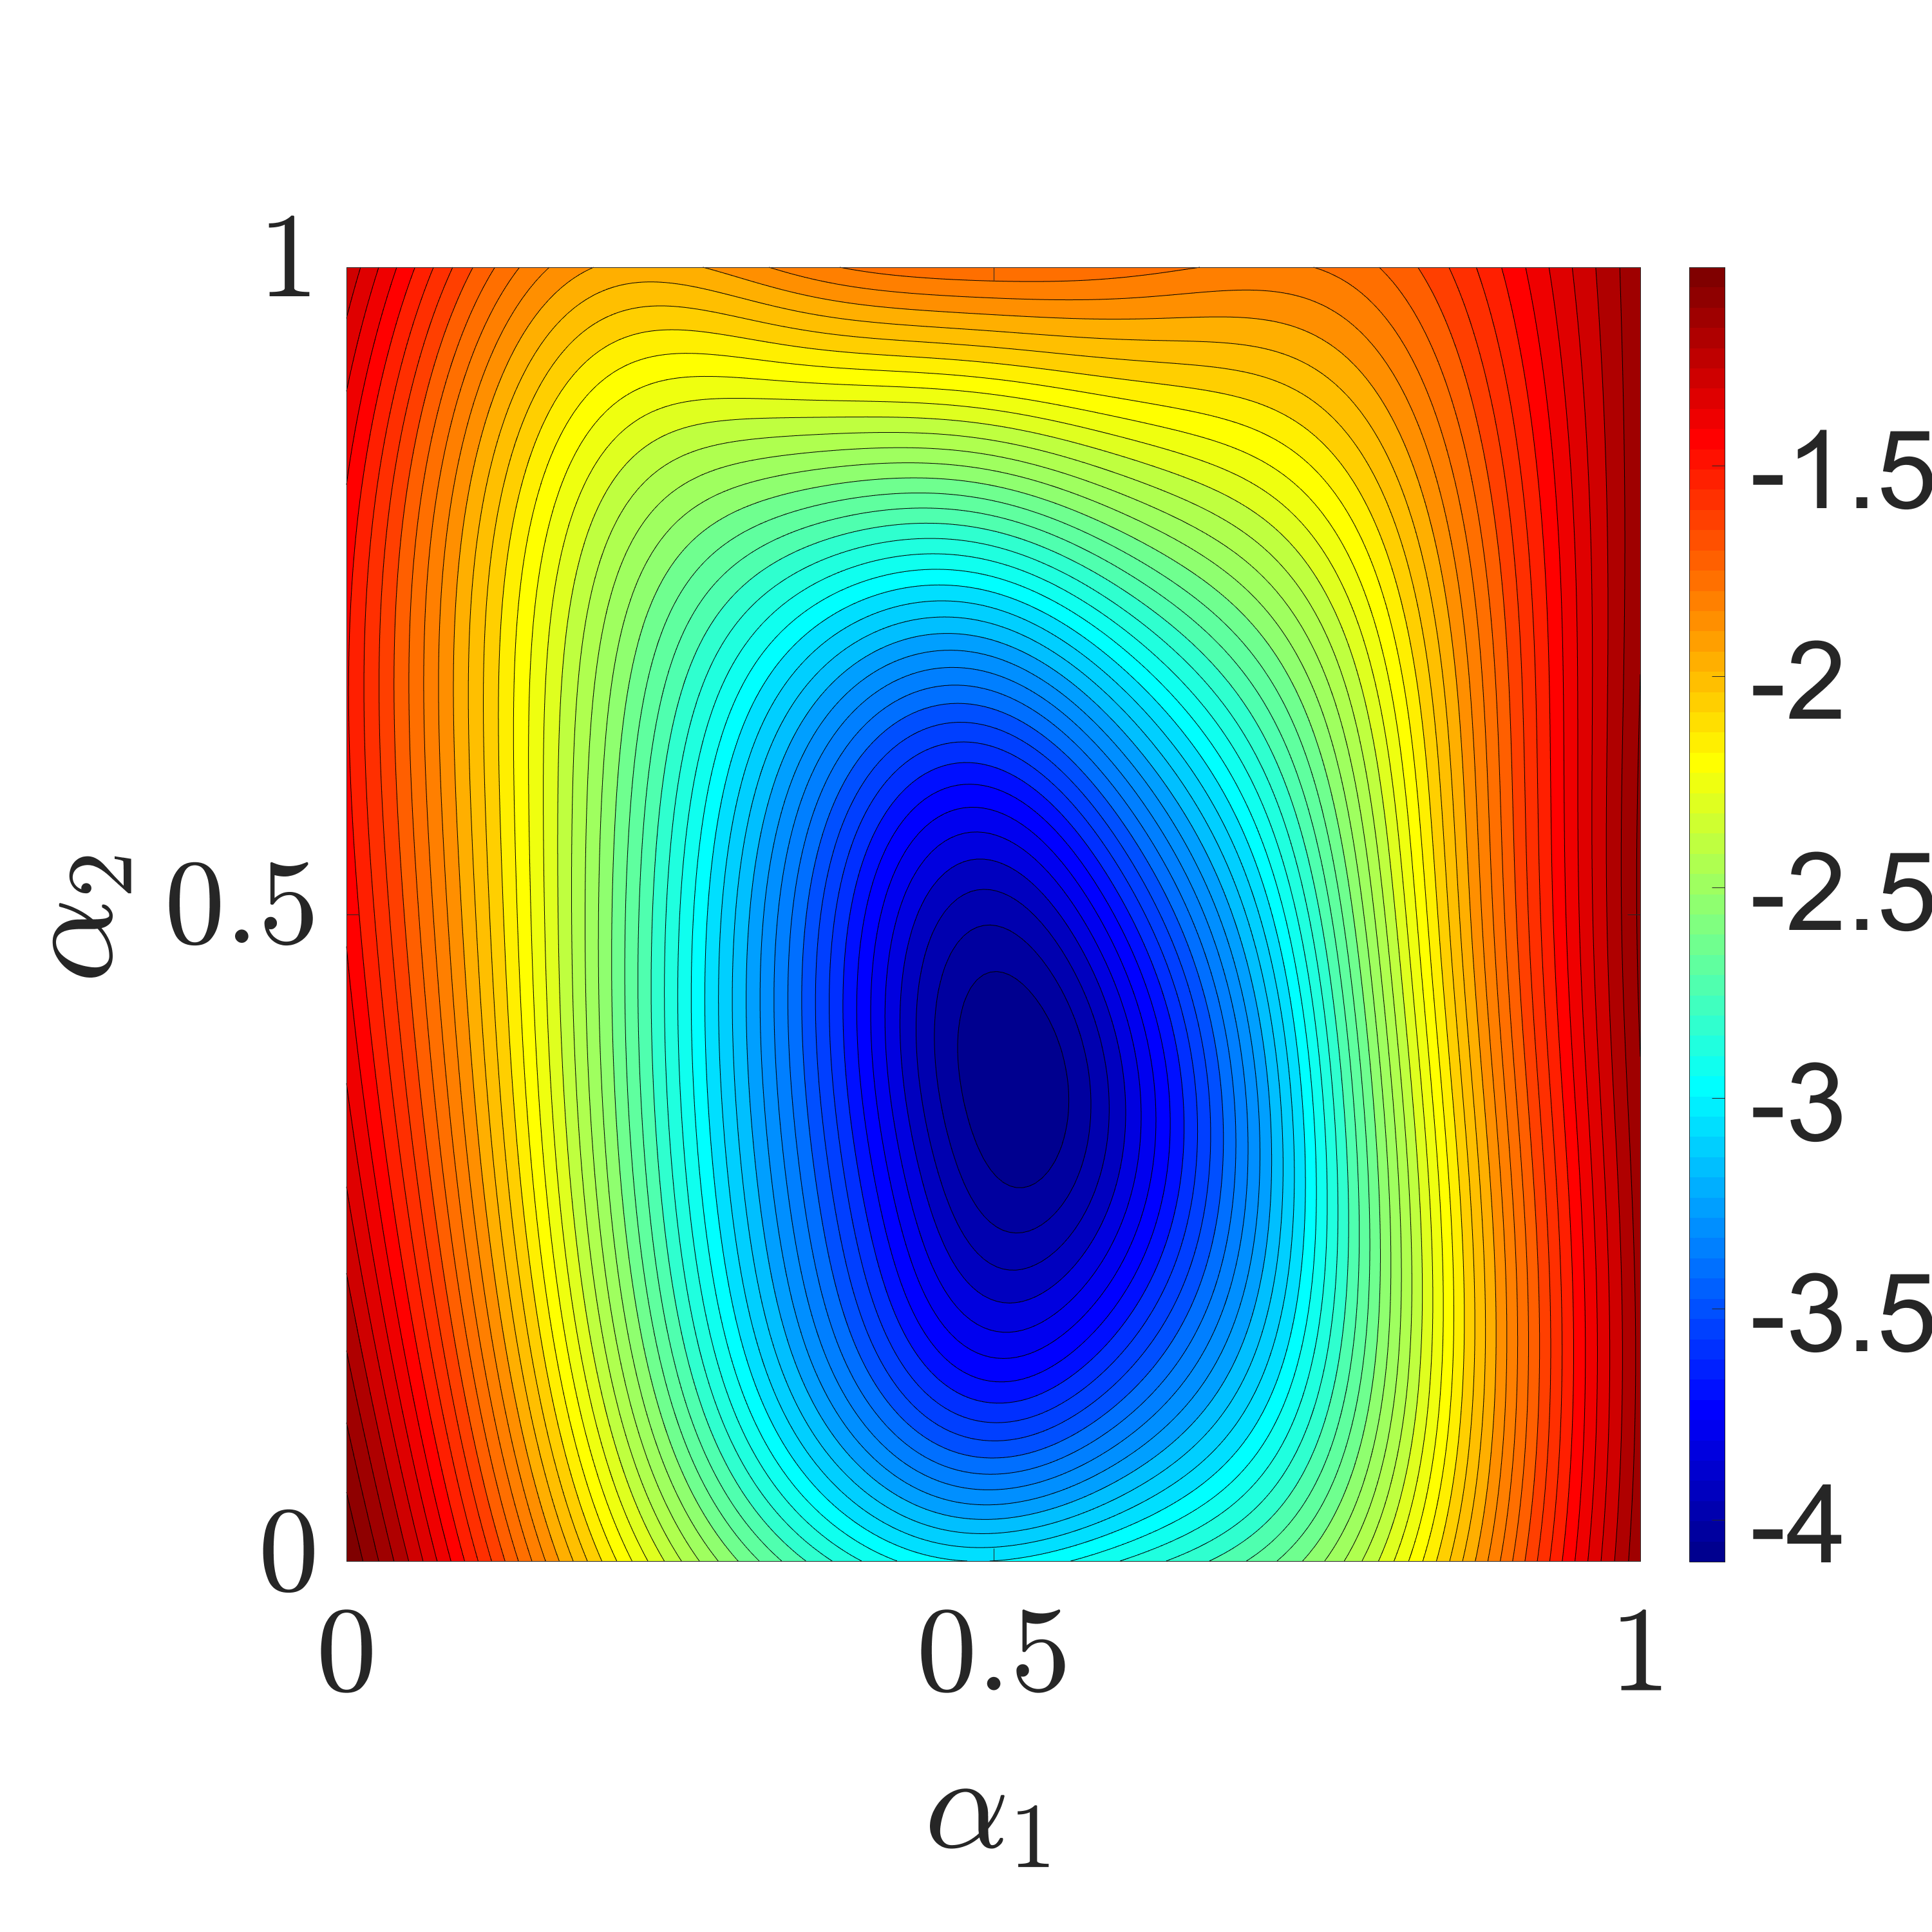
\includegraphics[height=0.88\textwidth]{tmax_1e6_model_3_contour_plot.pdf}
		\caption{Original}
	\end{subfigure}
	~\hspace{4pt}
	\begin{subfigure}[b]{0.32\textwidth}
		\centering
		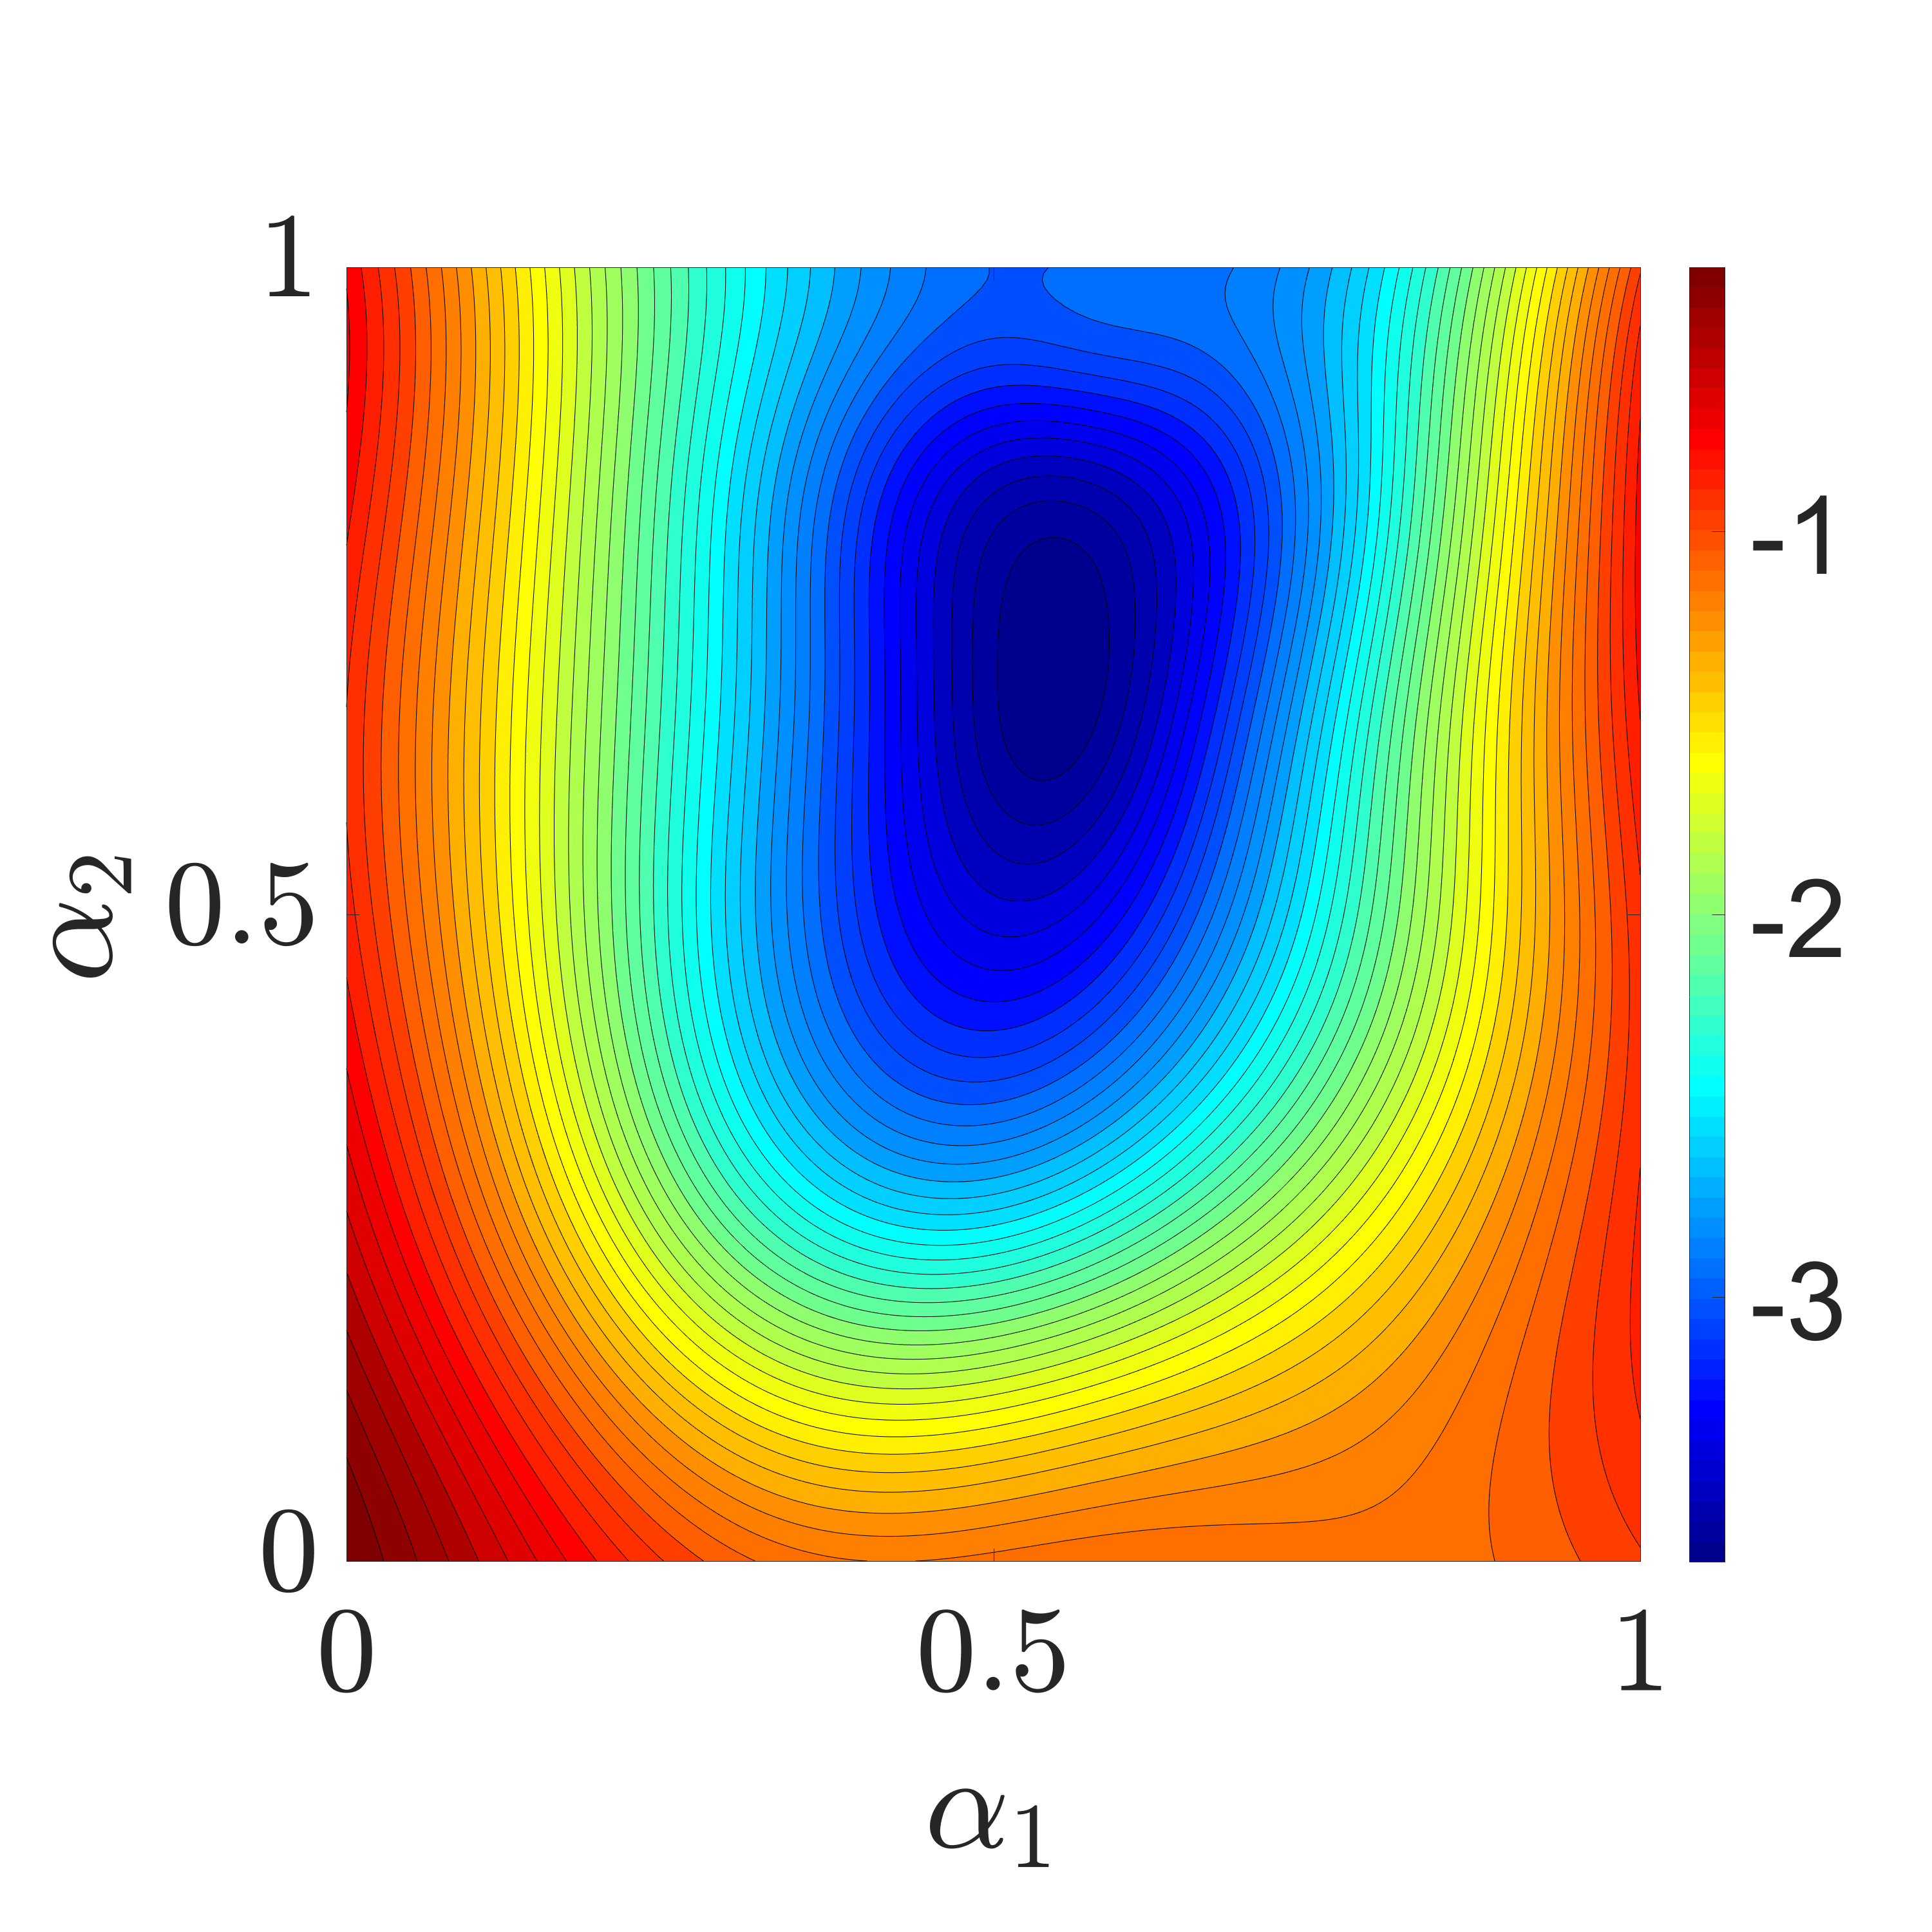
\includegraphics[height=0.88\textwidth]{tmax_1e6_model_2_contour_plot.pdf}
		\caption{First modification}
	\end{subfigure}
	~\hspace{-3pt}
	\begin{subfigure}[b]{0.32\textwidth}
		\centering
		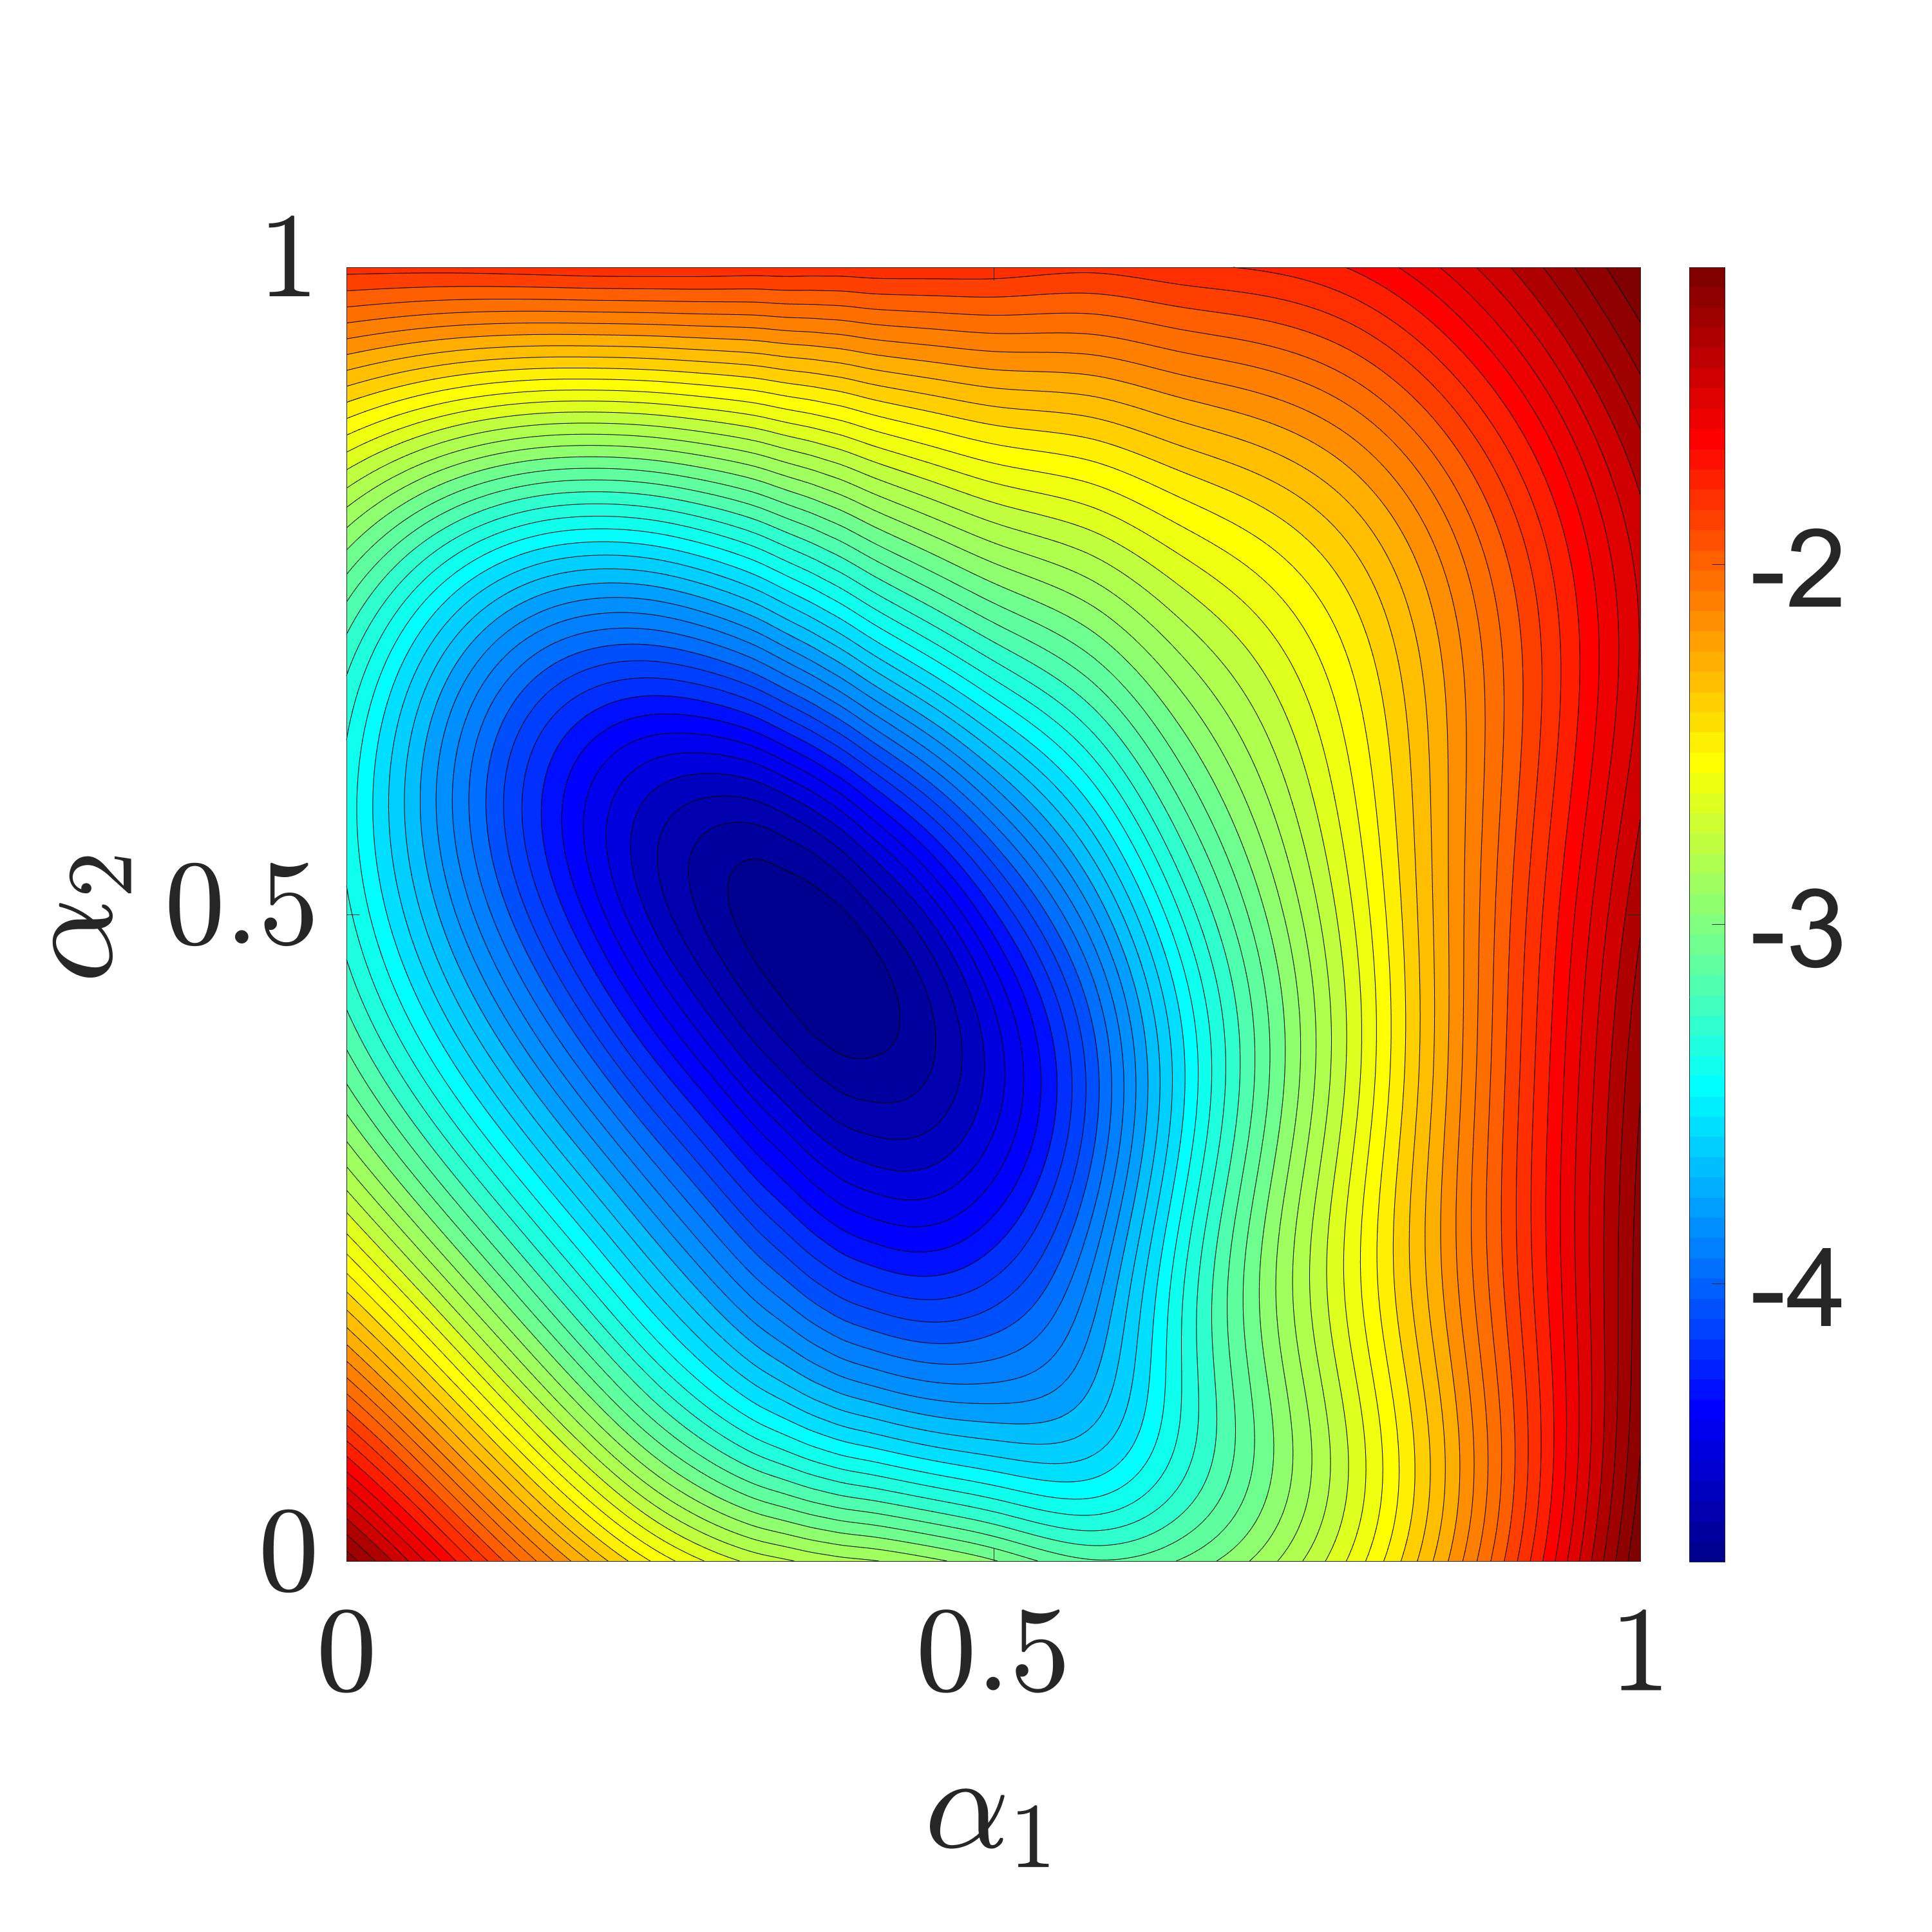
\includegraphics[height=0.88\textwidth]{tmax_1e6_model_4_contour_plot.pdf}
		\caption{Second modification}
	\end{subfigure}
	\caption{Contour plots of $\log_{10} \left(\E \left[(I_0-\gamma_0)^2\right]\right)$ (i.e. $\log_{10}$ MSE, estimated
		by averaging over $1000$ individual estimations)
		for different allocations of the sample budget $T=10^6$ between $N_0$, $N_1$,
		and $N_2$ for problem shown in~\eqref{eq:repeat-nest} and two modifications explained in
		the text.
		\label{fig:multi-tau}}
\end{figure}	

\subsection{Planning Cancer Treatment}
\label{sec:cancer}

We now introduce a real-world example to show the applicability of NMC in a scenario
where the solution is not analytically tractable and conventional MC is insufficient.
Consider a treatment center assessing a new policy for planning cancer treatments, subject to a budget. 
Clinicians must decide on a patient-by-patient basis whether to administer chemotherapy in the
hope that their tumor will reduce in size sufficiently to be able to perform surgery at a later date.
A treatment is considered to have been successful if the size of the tumor drops below a threshold value in a fixed time window.
The clinicians have at their disposal a simulator for the evolution of tumors with time,
parameterized by both observable values, $y$, such as tumor size, and unobservable values, $z$, such as the patient-specific response to treatment.
Given a set of input parameters, the simulator deterministically returns a binary response $\phi(y,z)\in\left\lbrace 0,1\right\rbrace $, with $\phi(y,z) = 1$ indicating a successful treatment.
To estimate the probability of a successful treatment for a given patient, the clinician must calculate the expected
success over these unobserved variables, namely $\E_{z\sim p(z|y)} [\phi(y,z)]$ where $p(z|y)$ represents a probabilistic
model for the unobserved variables, which could, for example, be constructed based on empirical data.
The clinician then decides whether to go ahead with the treatment for that
patient based on whether the calculated probability of success exceeds a certain threshold $T_{\mathrm{treat}}$.

The treatment center now wishes to estimate the expected number of patients that will be treated for a given $T_{\mathrm{treat}}$ so that it can minimize this threshold without exceeding its budget.
To do this, it needs to calculate the expectation of the clinician's decisions to administer 
treatment, giving the complete nested expectation for calculating the number of treated patients as
\begin{equation}
	\label{eq:cancer}
I(T_{\mathrm{treat}}) = \E_{y \sim p(y)} \left[\mathbb{I}\left(\E_{z\sim p(z|y)} [\phi(y,z)]>T_{\mathrm{treat}}\right)\right],
\end{equation}
where the identity function $\mathbb{I}(\cdot > T_{\mathrm{treat}})$ imposes a non-linear
mapping, such that conventional Monte Carlo estimation is not possible. Full details on $\phi$, $p(y)$, and $p(z|y)$ are 
provided in Appendix~\ref{sec:cancer_sim_app}.

To verify the convergence rate, we repeat the analysis from Section~\ref{sec:simple} for the problem defined 
by~\eqref{eq:cancer} at a fixed value of $T_{\mathrm{treat}}=0.35$. 
The results, shown in Figure~\ref{fig:emperical-conv-cancer}, again verify the theoretical rates. 
By further testing different values of $T_{\mathrm{treat}}$, we found $T_{\mathrm{treat}} \ge 0.125$ (i.e.
go ahead with treatment if the probability of success is 0.125 or greater) to be the optimal under the budget.

\subsection{Bayesian Experimental Design}
\label{sec:bo-design}

In this section we show how our results can be used to derive an improved estimator for the problem of
Bayesian experimental design (BED) in the case where the experiment outputs are discrete.  
In the interest of flow of the paper, we provide only a summary here, with a full introduction to BED, the derivation of all
the introduced estimators, and additional results provided in Appendix~\ref{sec:exp-design}.

\begin{figure}[t]
	\centering
	\begin{subfigure}[b]{0.49\textwidth}
		\centering
		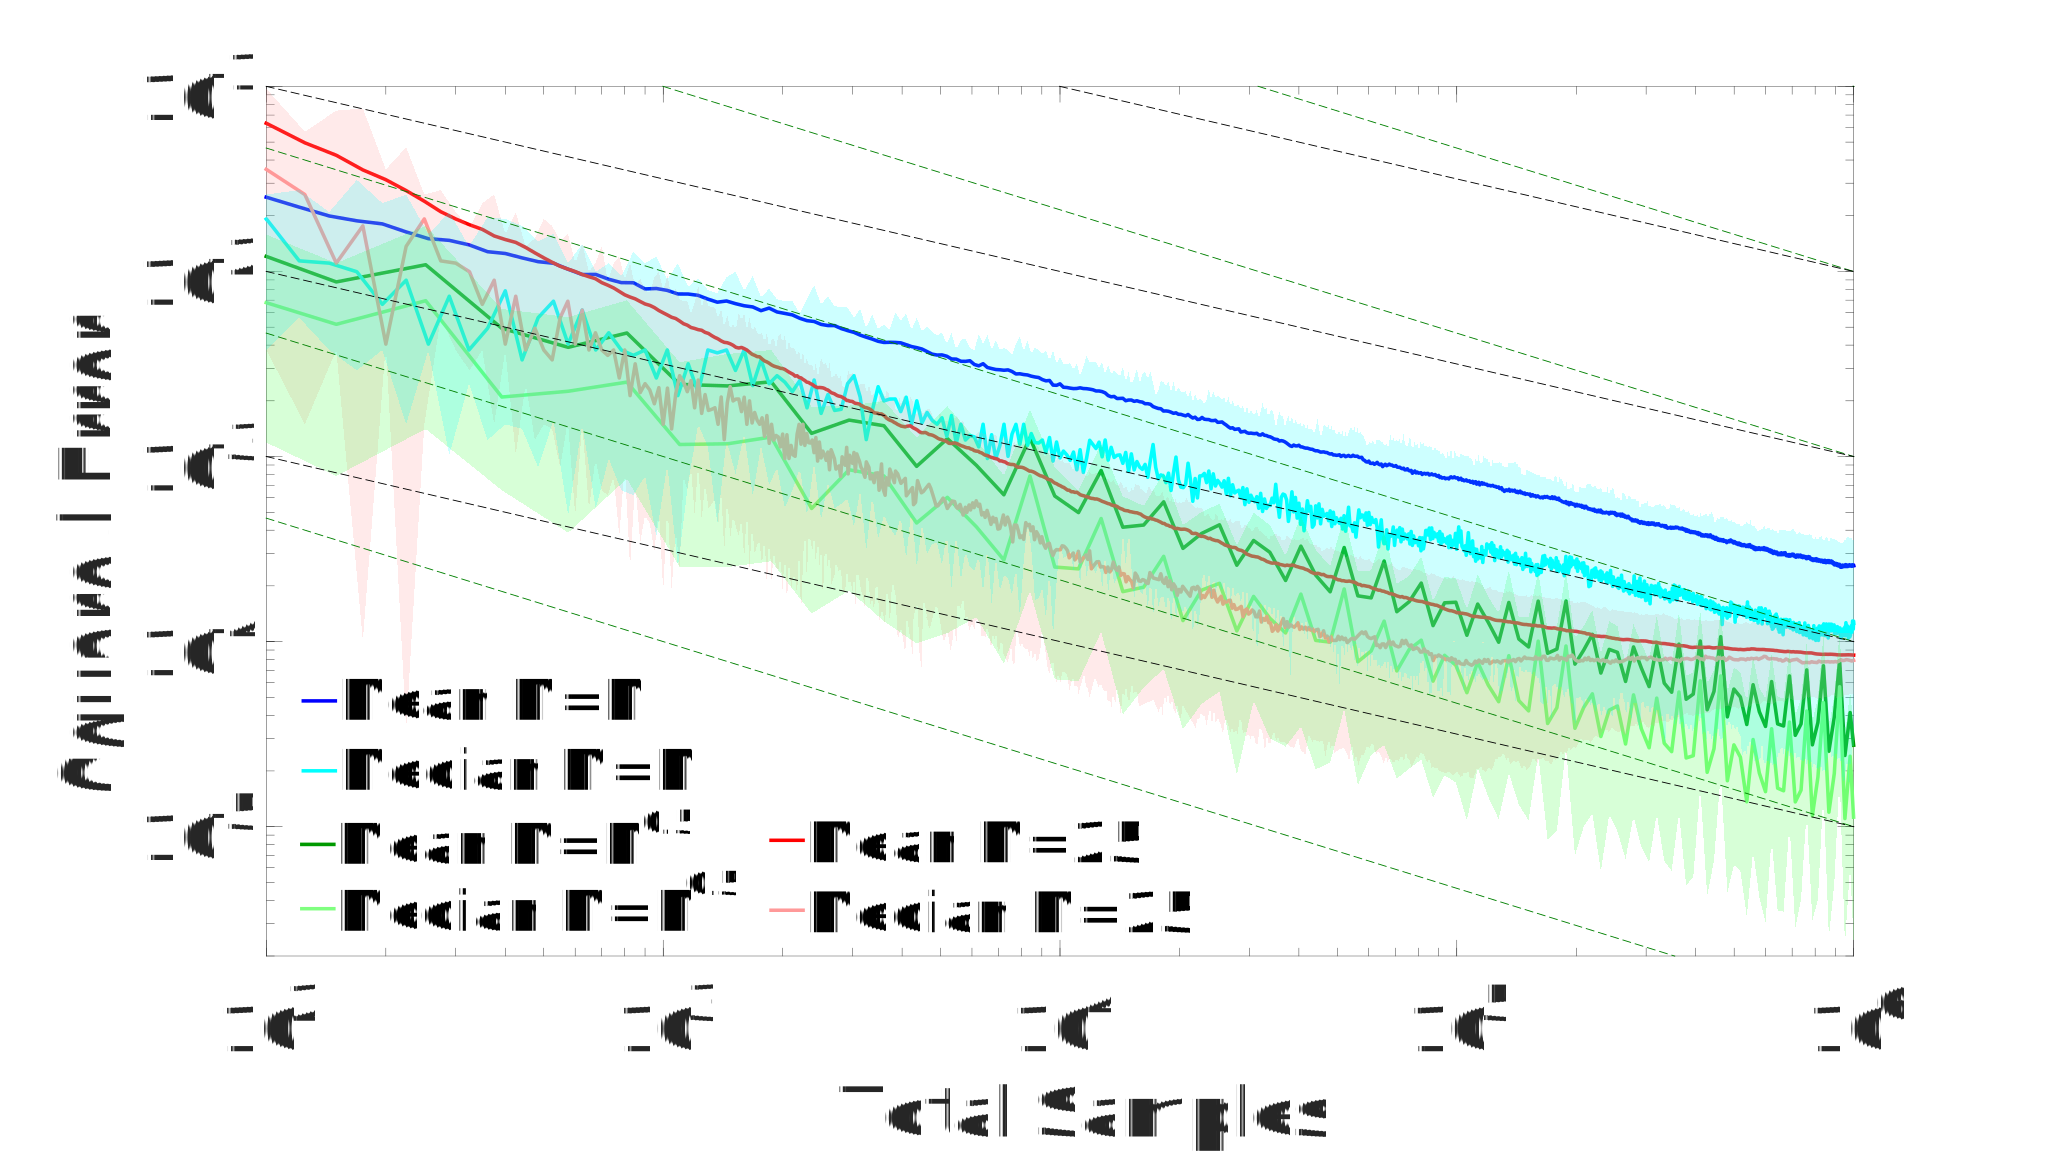
\includegraphics[width=0.99\textwidth,trim={1.5cm 0 3.5cm 0},clip]{canver_conv2}
		\caption{Cancer simulation\label{fig:emperical-conv-cancer}}
	\end{subfigure}
	\begin{subfigure}[b]{0.49\textwidth}
		\centering
		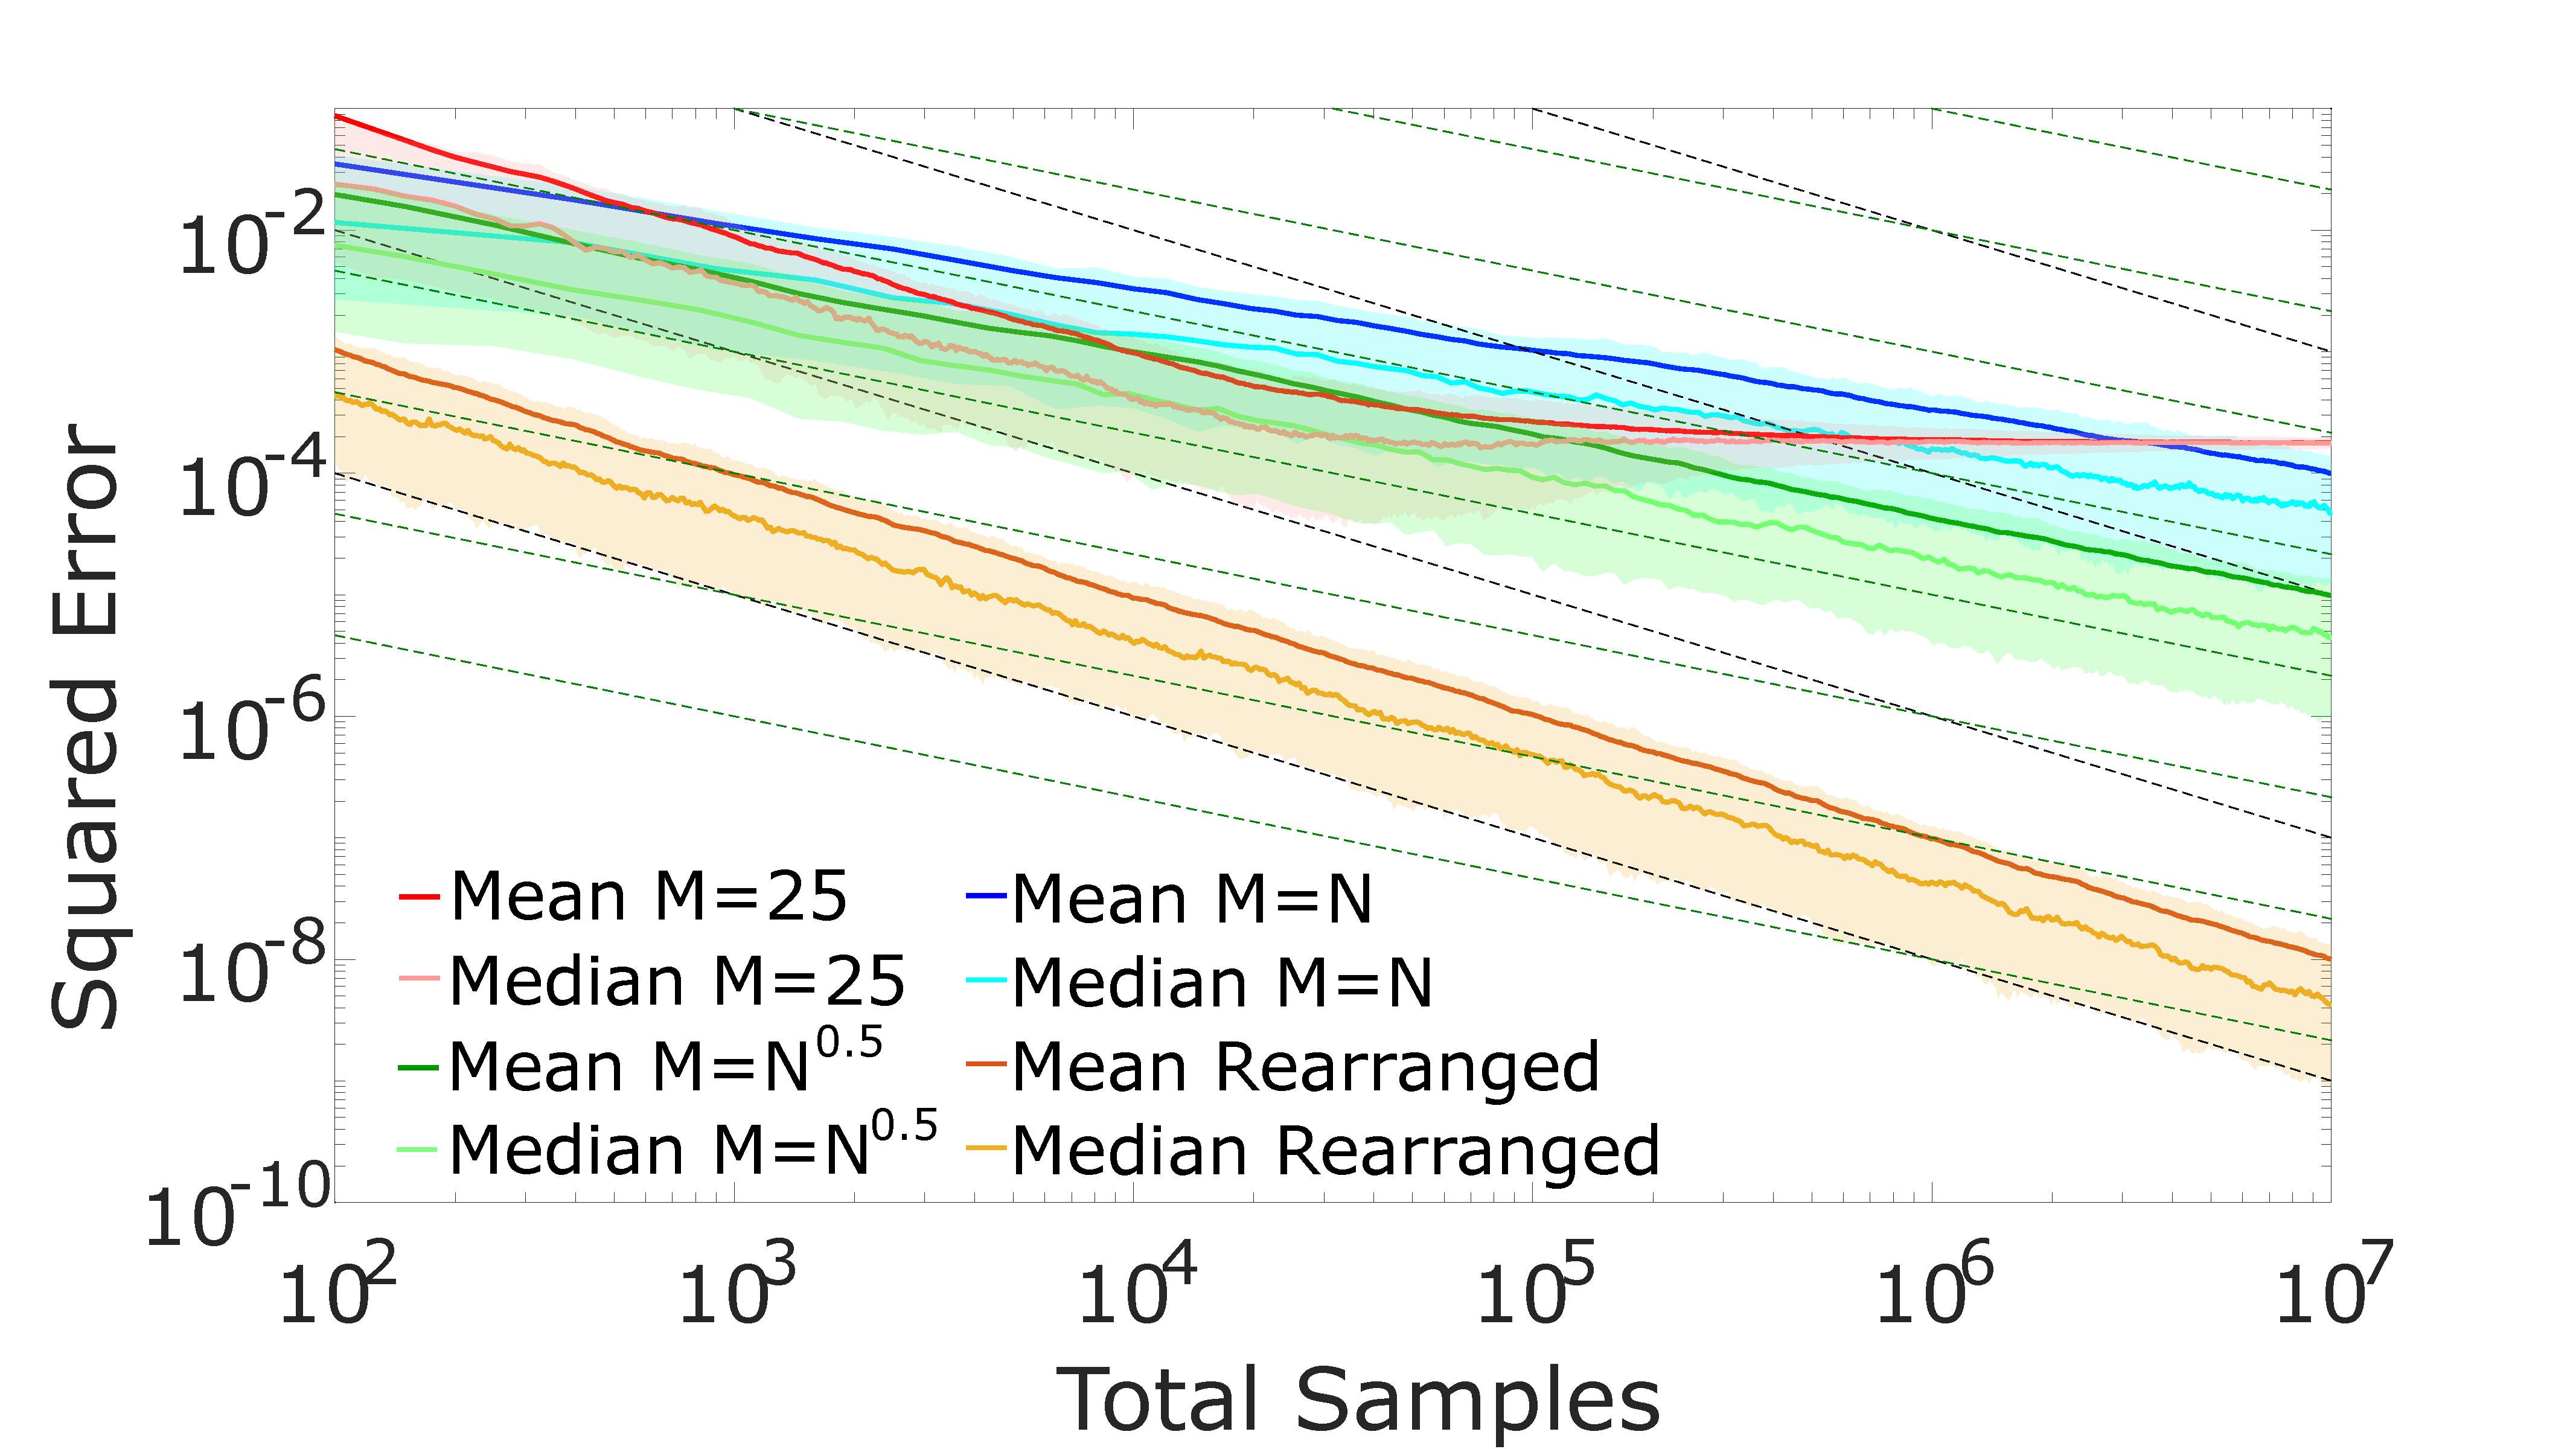
\includegraphics[width=0.99\textwidth,trim={1.5cm 0 3.5cm 0},clip]{exp_conv2}
		\caption{Bayesian experimental design\label{fig:exp-conv}}
	\end{subfigure}
	\caption{Convergence of NMC for cancer simulation (left) and of both NMC and our reformulated
		estimator~\eqref{eq:u_bar_MC_main} for the BED problem (right).
		A ground truth estimate for the cancer simulation was calculated
		using a single run with $M=10^5$ and $N=10^5$ and using a single run of the reformulated
		estimator with $10^{10}$ for the BED problem.
		Results are averaged over 1000 independent runs, while shaded regions give the 25\%-75\% quantiles. We
		see that the theoretical convergence rates are observed in all cases,
		with the advantages of the reformulated estimator particularly pronounced.
		On the cancer example when $M=\sqrt{N}$ an interesting fluctuation behavior is observed.  
		Further testing suggests that this originates because the bias of the estimator depends in
		a fluctuating manner on the value of $M$ as the binary output of $\phi(y,z)$ creates a quantization
		effect on the possible estimates for $\hat{\gamma}$.  This effect is also observed for the $M=N$ case,
		but is less pronounced. \vspace{-5pt}}
\end{figure}

Bayesian experimental design provides a framework for designing experiments in a manner that is optimal from
an information-theoretic viewpoint \citep{chaloner1995bayesian,sebastiani2000maximum}.  Given a prior
$p(\theta)$ on parameters $\theta$ and a corresponding likelihood $p(y|\theta,d)$ for experiment 
outcomes $y$ given a design $d$, the Bayesian optimal design $d^*$ is given by maximizing the mutual
information between $\theta$ and $y$ defined as follows
\begin{align}
\bar{U}(d)=
\int_{\mathcal{Y}}\int_{\Theta} p(y,\theta | d)\log\left(\frac{p(\theta |y, d)}{p(\theta)}\right)d\theta dy. 
\label{eq:u_bar_main}
\end{align}
Finding $d^*$ is challenging as the posterior $p(\theta |y, d)$ is rarely known in closed form.  
However, after appropriate algebraic manipulation, it can be shown that~\eqref{eq:u_bar_main}
is consistently estimated by
\begin{align}
\label{eq:exp-des-nmc-main}
\hat{U}_{\text{NMC}}(d) =
\frac{1}{N} \sum_{n=1}^{N} \left[ \log(p(y_n | \theta_{n,0},d)) 
- \log \left(\frac{1}{M} \sum_{m=1}^{M}p(y_n | \theta_{n,m},d)\right) \right]
\end{align}
where $\theta_{n,m} \sim p(\theta)$ for each $(m,n) \in \{0,\ldots,M\}\times \{1,\ldots,N\}$, 
and $y_n \sim p(y|\theta=\theta_{n,0}, d)$ for each $n \in \{1,\ldots,N\}$.  
This na\"{i}ve NMC estimator has been implicitly used by \cite{myung2013tutorial} and \cite{ouyang2016practical} amongst others and gives a convergence
rate of $O(1/M^2+1/N)$ as per Theorem~\ref{the:Repeat}.

When $y$ can only take on finitely many realizations $y_{1},\dots,y_c$, we use the ideas introduced
in Section~\ref{sec:discrete} to derive the following estimator
\begin{align}
\begin{split}
\label{eq:u_bar_MC_main}
\hat{U}_{R}(d) = &\frac{1}{N} \sum_{n=1}^{N} \sum_{c=1}^{C} p(y_c | \theta_n, d) \log\left(p(y_c | \theta_n, d)\right) \\
&- \sum_{c=1}^{C} \left[\left(\frac{1}{N}\sum_{n=1}^{N} p(y_c | \theta_n, d)\right) \log \left(\frac{1}{N} \sum_{n=1}^{N} p(y_c | \theta_n, d)\right) \right]
\end{split}
\end{align}
where $\theta_n \sim p(\theta)$ for each $n \in \{1,\dots,N\}$.  
As $C$ is a fixed
constant,~\eqref{eq:u_bar_MC_main} converges at the standard MC error rate of $O(1/N)$.  This constitutes
a substantially faster convergence as~\eqref{eq:exp-des-nmc-main} requires a total of $MN$
samples compared to $N$ for~\eqref{eq:u_bar_MC_main}.  To the best of our knowledge, this estimator for this experimental design problem with its superior convergence guarantee has not been introduced in the literature.

We finish by showing that the theoretical advantages of this reformulation also lead to empirical gains in the estimation of $\bar{U}(d)$.  For this we consider a model used in psychology experiments for delay discounting introduced by \cite{vincent2016hierarchical}, details of which are given in Appendix~\ref{sec:exp-design}.  Convergence results
shown in Figure~\ref{fig:exp-conv} demonstrate that the theoretical convergence rates
are observed while results given in Appendix~\ref{sec:exp-design} show that this leads to significant practical gains 
in estimating $\bar{U}(d)$.
